\iffalse
This file is protected by Copyright. Please refer to the COPYRIGHT file
distributed with this source distribution.

This file is part of OpenCPI <http://www.opencpi.org>

OpenCPI is free software: you can redistribute it and/or modify it under the
terms of the GNU Lesser General Public License as published by the Free Software
Foundation, either version 3 of the License, or (at your option) any later
version.

OpenCPI is distributed in the hope that it will be useful, but WITHOUT ANY
WARRANTY; without even the implied warranty of MERCHANTABILITY or FITNESS FOR A
PARTICULAR PURPOSE. See the GNU Lesser General Public License for more details.

You should have received a copy of the GNU Lesser General Public License along
with this program. If not, see <http://www.gnu.org/licenses/>.
\fi

%----------------------------------------------------------------------------------------
% Update the docTitle and docVersion per document
%----------------------------------------------------------------------------------------
\def\docTitle{OpenCPI\\Ettus E3XX Getting Started Guide}
\def\docVersion{1.5}
\def\rccplatform{xilinx13\_4}
\def\radioName{E310}
\def\mountPoint{/mnt/}
\def\copyLoc{<partition>}
%----------------------------------------------------------------------------------------
\documentclass{article}
\iffalse
This file is protected by Copyright. Please refer to the COPYRIGHT file
distributed with this source distribution.

This file is part of OpenCPI <http://www.opencpi.org>

OpenCPI is free software: you can redistribute it and/or modify it under the
terms of the GNU Lesser General Public License as published by the Free Software
Foundation, either version 3 of the License, or (at your option) any later
version.

OpenCPI is distributed in the hope that it will be useful, but WITHOUT ANY
WARRANTY; without even the implied warranty of MERCHANTABILITY or FITNESS FOR A
PARTICULAR PURPOSE. See the GNU Lesser General Public License for more details.

You should have received a copy of the GNU Lesser General Public License along
with this program. If not, see <http://www.gnu.org/licenses/>.
\fi
% Any changes to this document should be made in opencpi.git
\author{} % Force author to be blank
%----------------------------------------------------------------------------------------
% Paper size, orientation and margins
%----------------------------------------------------------------------------------------
\usepackage{geometry}
\geometry{
        letterpaper, % paper type
        portrait,    % text direction
        left=.75in,  % left margin
        top=.75in,   % top margin
        right=.75in, % right margin
        bottom=.75in % bottom margin
 }
%----------------------------------------------------------------------------------------
% Header/Footer
%----------------------------------------------------------------------------------------
\usepackage{fancyhdr} \pagestyle{fancy} % required for fancy headers
\renewcommand{\headrulewidth}{0.5pt}
\renewcommand{\footrulewidth}{0.5pt}
\rhead{\small{ANGRYVIPER Team}}
% \rfoot{\thepage}
%----------------------------------------------------------------------------------------
% Appendix packages
%----------------------------------------------------------------------------------------
\usepackage[toc,page]{appendix}
%----------------------------------------------------------------------------------------
% Defined Commands & Renamed Commands
%----------------------------------------------------------------------------------------
\renewcommand{\contentsname}{Table of Contents}
\renewcommand{\listfigurename}{List of Figures}
\renewcommand{\listtablename}{List of Tables}
\newcommand{\todo}[1]{\textcolor{red}{TODO: #1}\PackageWarning{TODO:}{#1}} % To do notes
\newcommand{\code}[1]{\texttt{#1}} % For inline code snippet or command line
%----------------------------------------------------------------------------------------
% Various packages
%----------------------------------------------------------------------------------------
\usepackage[usenames,dvipsnames]{xcolor} % for color names see https://en.wikibooks.org/wiki/LaTeX/Colors
\usepackage{hyperref}  % for linking urls and lists
\usepackage{graphicx}  % for including pictures by file
\usepackage{listings}  % for coding language styles
\usepackage{rotating}  % for sideways table
\usepackage{pifont}    % for sideways table
\usepackage{pdflscape} % for landscape view
\usepackage{subfig}
\hyphenation{ANGRY-VIPER} % Tell it where to hyphenate
\hyphenation{Cent-OS} % Tell it where to hyphenate
\hyphenation{install-ation} % Tell it where to hyphenate
\uchyph=0 % Never hyphenate acronyms like RCC (I think this overrides ANGRYVIPER above)
\renewcommand\_{\textunderscore\allowbreak} % Allow words to break/newline on underscores
%----------------------------------------------------------------------------------------
% Table packages
%----------------------------------------------------------------------------------------
\usepackage{longtable} % for long possibly multi-page tables
\usepackage{tabularx} % c=center,l=left,r=right,X=fill
% These define tabularx columns "C" and "R" to match "X" but center/right aligned
\newcolumntype{C}{>{\centering\arraybackslash}X}
\newcolumntype{R}{>{\raggedleft\arraybackslash}X}
\usepackage{float}
\floatstyle{plaintop}
\usepackage[tableposition=top]{caption}
\newcolumntype{P}[1]{>{\centering\arraybackslash}p{#1}}
\newcolumntype{M}[1]{>{\centering\arraybackslash}m{#1}}
%----------------------------------------------------------------------------------------
% Block Diagram / FSM Drawings
%----------------------------------------------------------------------------------------
\usepackage{tikz}
\usetikzlibrary{shapes,arrows,fit,positioning}
\usetikzlibrary{automata} % used for the fsm
%----------------------------------------------------------------------------------------
% Colors Used
%----------------------------------------------------------------------------------------
\usepackage{colortbl}
\definecolor{blue}{rgb}{.7,.8,.9}
\definecolor{ceruleanblue}{rgb}{0.16, 0.32, 0.75}
\definecolor{drkgreen}{rgb}{0,0.6,0}
\definecolor{deepmagenta}{rgb}{0.8, 0.0, 0.8}
\definecolor{cyan}{rgb}{0.0,0.6,0.6}
\definecolor{maroon}{rgb}{0.5,0,0}
%----------------------------------------------------------------------------------------
% VHDL Coding Language Style
% modified from: http://latex-community.org/forum/viewtopic.php?f=44&t=22076
%----------------------------------------------------------------------------------------
\lstdefinelanguage{VHDL}
{
        basicstyle=\ttfamily\footnotesize,
        columns=fullflexible,keepspaces,      % https://tex.stackexchange.com/a/46695/87531
        keywordstyle=\color{ceruleanblue},
        commentstyle=\color{drkgreen},
        morekeywords={
    library,use,all,entity,is,port,in,out,end,architecture,of,
    begin,and, signal, when, if, else, process, end,
        },
        morecomment=[l]--
}
%----------------------------------------------------------------------------------------
% XML Coding Language Style
% modified from: http://tex.stackexchange.com/questions/10255/xml-syntax-highlighting
%----------------------------------------------------------------------------------------
\lstdefinelanguage{XML}
{
        basicstyle=\ttfamily\footnotesize,
        columns=fullflexible,keepspaces,
        morestring=[s]{"}{"},
        morecomment=[s]{!--}{--},
        commentstyle=\color{drkgreen},
        moredelim=[s][\color{black}]{>}{<},
        moredelim=[s][\color{cyan}]{\ }{=},
        stringstyle=\color{maroon},
        identifierstyle=\color{ceruleanblue}
}
%----------------------------------------------------------------------------------------
% DIFF Coding Language Style
% modified from http://tex.stackexchange.com/questions/50176/highlighting-a-diff-file
%----------------------------------------------------------------------------------------
\lstdefinelanguage{diff}
{
        basicstyle=\ttfamily\footnotesize,
        columns=fullflexible,keepspaces,
        breaklines=true,                                % wrap text
        morecomment=[f][\color{ceruleanblue}]{@@},      % group identifier
        morecomment=[f][\color{red}]-,                  % deleted lines
        morecomment=[f][\color{drkgreen}]+,             % added lines
        morecomment=[f][\color{deepmagenta}]{---},      % Diff header lines (must appear after +,-)
        morecomment=[f][\color{deepmagenta}]{+++},
}
%----------------------------------------------------------------------------------------
% Python Coding Language Style
% modified from
%----------------------------------------------------------------------------------------
\lstdefinelanguage{python}
{
        basicstyle=\ttfamily\footnotesize,
        columns=fullflexible,keepspaces,
        keywordstyle=\color{ceruleanblue},
        commentstyle=\color{drkgreen},
        stringstyle=\color{orange},
        morekeywords={
    print, if, sys, len, from, import, as, open,close, def, main, for, else, write, read, range,
        },
        comment=[l]{\#}
}
%----------------------------------------------------------------------------------------
% Fontsize Notes in order from smallest to largest
%----------------------------------------------------------------------------------------
%    \tiny
%    \scriptsize
%    \footnotesize
%    \small
%    \normalsize
%    \large
%    \Large
%    \LARGE
%    \huge
%    \Huge

\iffalse
This file is protected by Copyright. Please refer to the COPYRIGHT file
distributed with this source distribution.

This file is part of OpenCPI <http://www.opencpi.org>

OpenCPI is free software: you can redistribute it and/or modify it under the
terms of the GNU Lesser General Public License as published by the Free Software
Foundation, either version 3 of the License, or (at your option) any later
version.

OpenCPI is distributed in the hope that it will be useful, but WITHOUT ANY
WARRANTY; without even the implied warranty of MERCHANTABILITY or FITNESS FOR A
PARTICULAR PURPOSE. See the GNU Lesser General Public License for more details.

You should have received a copy of the GNU Lesser General Public License along
with this program. If not, see <http://www.gnu.org/licenses/>.
\fi

\iffalse

This snippet defines macros to be used when describing ocpidev commands
to give the user the equivalent in the IDE. See AV-4628.

To see all output:
\code{\$ ocpidev build something something}
\OcpidevBuild
\code{\$ ocpidev clean something something}
\OcpidevClean
\code{\$ ocpidev run test something something}
\OcpidevRunTest
\code{\$ ocpidev create (no options)}
\OcpidevCreate{}
\code{\$ ocpidev create project}
\OcpidevCreate{Project}
\code{\$ ocpidev clean project Project}
\OcpidevCleanProject{Project}
\code{\$ ocpidev register project my\_proj}
\OcpidevRegisterProject{my_proj}
\code{\$ ocpidev unregister project my\_proj}
\OcpidevUnRegisterProject{my_proj}

\fi
% https://tex.stackexchange.com/a/5227
\usetikzlibrary{shadows}
\newcommand*\OcpidevKeystroke[1]{%
  \tikz[baseline=(key.base)]
    \node[%
      draw,
      fill=white,
      drop shadow={shadow xshift=0.25ex,shadow yshift=-0.25ex,fill=black,opacity=0.75},
      rectangle,
      rounded corners=2pt,
      inner sep=1pt,
      line width=0.5pt,
      font=\scriptsize\sffamily
    ](key) {#1\strut}
  ;
}

\providecommand{\OcpidevCtrlClick}{(use \OcpidevKeystroke{~Ctrl~} for multiple selection)}

\providecommand{\OcpidevTemplate}[1]{
\begin{center}
\framebox{\parbox{0.8\linewidth}{\textit{To perform this operation within the IDE:}
#1}}
\end{center}
}

% OcpidevBuild = "ocpidev build"
\providecommand{\OcpidevBuild}{\OcpidevTemplate{
\begin{enumerate}
\setlength\itemsep{0em} %tighten
\item Open the ANGRYVIPER Perspective
\item Select the asset from OpenCPI Project View
\item Import to AV Operations Panel using ``$>$'' button
\item Select the RCC and/or HDL platforms for the build \OcpidevCtrlClick
\item Click ``Build''
\end{enumerate}
% Open the ANGRYVIPER Perspective, select the RCC and/or HDL platforms for the build \OcpidevCtrlClick , then select the asset in OpenCPI Projects view, right click, select build.
}}

% OcpidevClean = "ocpidev clean"
\providecommand{\OcpidevClean}{\OcpidevTemplate{
In the OpenCPI Projects view, select the project, right-click, select clean from the menu.
}}

% OcpidevRunTest = "ocpidev run test"
\providecommand{\OcpidevRunTest}{\OcpidevTemplate{
\begin{enumerate}
\setlength\itemsep{0em} %tighten
\item Click the ``Tests'' radio button and select RCC and/or HDL platforms for the run \OcpidevCtrlClick .
\item Click the ``+remotes'' button, enter the remote string, click OK.
\item Select the remote in the remotes list.
\item In the OpenCPI Projects view, select the desired unit tests, click the ``$>$'' button in the operations panel, then click the desired operation to build and then run the listed tests on the selected remote.
\end{enumerate}
}}

% OcpidevCreate = "ocpidev create <$1>"
\providecommand{\OcpidevCreate}[1]{\OcpidevTemplate{
\begin{itemize}
\setlength\itemsep{0em} %tighten
\item Place the cursor in the OpenCPI Projects panel, right click, select asset wizard.
\item Select the asset type\ifthenelse{\equal{#1}{}}{}{ (``#1'')} in the drop-down, fill in the required inputs, click finish.
\item When the process finishes, the new asset is displayed in both project views. (If the asset has an XML editor, then the editor opens.)
\end{itemize}
}}

% OcpidevCleanProject = "ocpidev clean project <$1>"
\providecommand{\OcpidevCleanProject}[1]{\OcpidevTemplate{\textit{(The project ``#1'' must be imported into the IDE and then refresh the OpenCPI Projects view so the project is shown.)}
\begin{itemize}
\setlength\itemsep{0em} %tighten
\item Right click on #1 $\Rightarrow$ ``Clean''
\end{itemize}
}}

% OcpidevRegisterProject = "ocpidev register project <$1>"
% OcpidevUnRegisterProject = "ocpidev unregister project <$1>"
\providecommand{\OcpidevRegisterProjectKernel}[2]{\OcpidevTemplate{\textit{(The project ``#1'' must be imported into the IDE and then refresh the OpenCPI Projects view so the project is shown.)}
\begin{itemize}
\setlength\itemsep{0em} %tighten
\item In the OpenCPI Projects view, select the project, right-click, select ``#2'' from the menu. (Depending on state of the project, this option may not be available.)
\end{itemize}
}}
\providecommand{\OcpidevRegisterProject}[2]{\OcpidevRegisterProjectKernel{\path{#1}}{register}}
\providecommand{\OcpidevUnRegisterProject}[2]{\OcpidevRegisterProjectKernel{\path{#1}}{unregister}}

\date{Version \docVersion} % Force date to be blank and override date with version
\title{\docTitle}
\lhead{Ettus E3XX Getting Started Guide}
%----------------------------------------------------------------------------------------
\usepackage[T1]{fontenc} % http://tex.stackexchange.com/a/181119
\usepackage{graphicx}
\graphicspath{ {figures/} }
\lstset{ % https://tex.stackexchange.com/a/116572
  basicstyle=\ttfamily,
  columns=fullflexible,
  % frame=single,
  breaklines=true,
  showstringspaces=true,
  showspaces=true,
  postbreak=\mbox{\textcolor{red}{$\hookrightarrow$}\space},
}
\begin{document}
\maketitle
\begin{figure}[H]
 \centering
 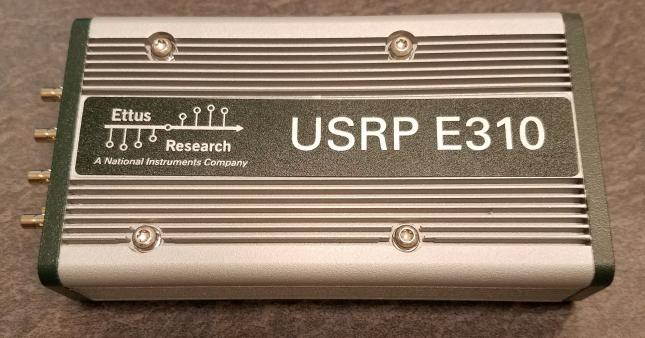
\includegraphics[scale=0.9]{img/top.jpg}
 \caption{Top View (E310)}
 \label{fig:top}
\end{figure}
%\thispagestyle{fancy}
\newpage

	\begin{center}
	\textit{\textbf{Revision History}}
		\begin{table}[H]
		\label{table:revisions} % Add "[H]" to force placement of table
			\begin{tabularx}{\textwidth}{|c|X|l|}
			\hline
			\rowcolor{blue}
			\textbf{Revision} & \textbf{Description of Change} & \textbf{Date} \\
		    \hline
		    v1.3.1-E3XX & Initial Release & 3/2018 \\
			\hline
		    v1.4 & Updated for Release & 9/2018 \\
			\hline
		    v1.5 & Version bump only & 4/2019 \\
			\hline
			\end{tabularx}
		\end{table}
	\end{center}

\newpage

\tableofcontents

\newpage

\section{References}
	This document assumes a basic understanding of the Linux command line (or ``shell'') environment.  The reference(s) in Table 1 can be used as an overview of OpenCPI and may prove useful.

\def\refcapbottom{}
\iffalse
This file is protected by Copyright. Please refer to the COPYRIGHT file
distributed with this source distribution.

This file is part of OpenCPI <http://www.opencpi.org>

OpenCPI is free software: you can redistribute it and/or modify it under the
terms of the GNU Lesser General Public License as published by the Free Software
Foundation, either version 3 of the License, or (at your option) any later
version.

OpenCPI is distributed in the hope that it will be useful, but WITHOUT ANY
WARRANTY; without even the implied warranty of MERCHANTABILITY or FITNESS FOR A
PARTICULAR PURPOSE. See the GNU Lesser General Public License for more details.

You should have received a copy of the GNU Lesser General Public License along
with this program. If not, see <http://www.gnu.org/licenses/>.
\fi

% This snippet creates the "References" table labeled "table:references"
% It creates three columns: Name, Publisher, Link and then inserts default documents
%
% To skip these defaults, define macros named
% refskipgs to skip "Getting Started"
% refskipig to skip "Installation Guide"
% refskipac to skip "Acronyms and Definitions"
% refskipocpiov to skip "OpenCPI Overview"
%
% See RPM_Installation_Guide.tex for examples
%
% After the defaults, it optionally inserts the "myreferences" macro that
% you defined elsewhere (you put hlines above all lines)
%
% If you want the \caption on the bottom, define "refcapbottom"
\begin{center}
\renewcommand*\footnoterule{} % Remove separator line from footnote
\renewcommand{\thempfootnote}{\arabic{mpfootnote}} % Use Arabic numbers (or can't reuse)
\begin{minipage}{0.9\textwidth}
  \begin{table}[H]
\ifx\refcapbottom\undefined
  \caption {References}
  \label{table:references}
\fi
  \begin{tabularx}{\textwidth}{|C|c|C|}
    \hline
    \rowcolor{blue}
    \textbf{Title} & \textbf{Published By} & \textbf{Link} \\
\ifx\refskipgs\undefined
    \hline
    Getting Started & ANGRYVIPER Team & \path{Getting_Started.pdf} \\
\fi
\ifx\refskipig\undefined
    \hline
    Installation Guide & ANGRYVIPER Team & \path{RPM_Installation_Guide.pdf} \\
\fi
\ifx\refskipac\undefined
    \hline
    Acronyms and Definitions & ANGRYVIPER Team & \path{Acronyms_and_Definitions.pdf} \\
\fi
\ifx\refskipocpiov\undefined
    \hline
    Overview & OpenCPI &
% Analytics: https://goo.gl/info/RskxiV
\url{https://goo.gl/RskxiV} \\
\fi
\ifx\myreferences\undefined
\else
    \myreferences
\fi
    \hline
  \end{tabularx}
\ifx\refcapbottom\undefined
\else
  \caption {References}
  \label{table:references}
\fi
  \end{table}
\end{minipage}
\end{center}


\newpage
\section{Overview}
This document provides steps for configuring a factory provided Ettus USRP E310 with the OpenCPI runtime environment for executing applications, configuring a development system to build OpenCPI bitstreams targeting the \textit{e3xx} platform, and examples of executing applications on the OpenCPI configured E310.

\section{Prerequisites}
\begin{flushleft}
This guide assumes that, at a minimum, the following RPMs are installed:  \\
\begin{table}[H]
	\label{table:rpms}
		\begin{tabularx}{\textwidth}{|c|X|}
		\hline
		\rowcolor{blue}
		\textbf{RPM Name} & \textbf{Description} \\
		\hline
		\hline
		All prerequisite RPMs & These packages have OpenCPI-specific patches and are provided as RPMs. This packaging ensures they will not conflict with other installed copies by using a nonstandard installation location of \path{/opt/opencpi/prerequisites}. \\
		\hline
		\small{\code{angryviper-ide-*.x86 64.rpm}} &
		The ANGRYVIPER IDE (Eclipse with plugins). See RPM Installation Guide.pdf, Appendix D for an alternative method to set up the IDE using an existing Eclipse installation. \\			
		\hline
		\small{\code{opencpi-*.x86\_64.rpm}} &
		Base installation RPM includes the runtime portion of the Component
Development Kit (CDK) and the source for the ocpi.core and ocpi.assets Projects containing framework essential components, workers,
platforms, etc. \\
		\hline
		\small{\code{opencpi-devel-*.x86\_64.rpm}} &
		Additional header files and scripts for developing new assets as HDL
and/or RCC. \\
		\hline
		\small{\code{opencpi-sw-platform-xilinx13\_4-*.noarch.rpm}} &
		Additional files necessary to build the framework targeting specific
RCC/software platforms, independent of the final deployed hardware. \\
		\hline
		\path{opencpi-hw-platform-e3xx-*.noarch.rpm} &
		Additional files necessary to build the framework targeting specific hard-ware platform "X" when running RCC platform "Y" ("Y" can be "no sw"). This RPM also includes hardware-specific SD Card images when applicable. \\
		\hline		
	\end{tabularx}
\end{table}

	\subsection{Installation of provided projects: \textit{core}, \textit{assets} and \textit{bsp\_e310}}
	This guide  assumes the user has executed \textit{ocpi-copy-projects}, accepting the default settings, to copy and register the \textit{core}, \textit{assets}, and \textit{bsp\_e310} projects from the /opt/opencpi/projects for building bitstreams for the E310. Reference the Getting Started Guide for details on \textit{ocpi-copy-projects}.  Although the projects are registered by \textit{ocpi-copy-projects}, changes to the registry can be made via \code{ocpidev un/register project} or the ANGRYVIPER GUI.\medskip

\begin{verbatim}
$ ocpi-copy-projects
...
$ ls ~/ocpi_projects
assets bsp_e310 core
$ ocpidev show registry
Project registry is located at: /opt/opencpi/cdk/../project-registry
----------------------------------------------------------------------------------------
| Project Package-ID  | Path to Project                                 | Valid/Exists |
| ------------------  | ---------------                                 | ------------ |
| ocpi.core           | /home/<user>/ocpi_projects/core                   | True         |
| ocpi.assets         | /home/<user>/ocpi_projects/assets                 | True         |
| ocpi.bsp.e310       | /home/<user>/ocpi_projects/bsp_e310               | True         |
----------------------------------------------------------------------------------------
\end{verbatim}

\subsection{Vendor Software Setup}
The platform that is expected to be used is the Ettus Research/National Instruments Universal Software Radio Peripheral (USRP) E310 (or E3XX) SDR (\textit{e.g.} e3xx). This OpenCPI-enabled platform provides the capability of deploying hardware and software workers while using Xilinx's 13.4 distribution of Linux.\\ \bigskip

The synthesizers and cross-compilers required to build HDL and RCC Workers for this Platform are installed by following the instructions found in the \textit{OpenCPI FPGA Vendor Tools Installation Guide}. This document assumes that the user has installed the appropriate versions of Vivado and the Xilinx SDK.\\ \bigskip

\subsection{Building Required Projects}
\label{sec:Building OpenCPI projects}
The \textit{core}, \textit{assets}, and \textit{bsp\_e310} projects must be built \textit{in a specific order} for this platform. This section outlines how to build the relevant projects and provides the commands to do so.\medskip

For this document, the projects should be built as follows:\\

\begin{enumerate}
	\item Build \code{core} for the \code{xilinx13\_4} RCC Platform and the \code{e3xx} HDL Platform, but omit assemblies
	\item Build \code{assets} for the \code{xilinx13\_4} RCC Platform and the \code{e3xx} HDL Platform, but omit assemblies
	\item Build the \code{bsp\_e310} project for these same platforms
	\item Build the \code{testbias} assembly from the \code{assets} project. This will be used later in this guide.
		\subitem Once the HDL Platform is built in the BSP project, assemblies can be built for that HDL platform
\end{enumerate}
\begin{lstlisting}[showspaces=false]
$ cd /home/<user>/ocpi_projects/ && \
$ ocpidev build -d core     --rcc-platform xilinx13_4 --hdl-platform e3xx --no-assemblies && \
$ ocpidev build -d assets   --rcc-platform xilinx13_4 --hdl-platform e3xx --no-assemblies && \
$ ocpidev build -d bsp_e310 --rcc-platform xilinx13_4 --hdl-platform e3xx && \
$ ocpidev build -d assets hdl assembly testbias       --hdl-platform e3xx;
\end{lstlisting}
Note: replace ``\code{<user>}'' with your username in the commands above.\\\medskip

Each of these build commands can also be performed via the ANGRYVIPER IDE as follows:
\OcpidevBuild
See the ANGRYVIPER Team's Getting Started Guide for additional information concerning the use of \code{ocpidev} and the ANGRYVIPER IDE to build OpenCPI assets.

\subsection{Hardware Setup}
\begin{itemize}
\item \textbf{Ettus USRP E3XX}\\ \medskip
It is expected that this SDR package includes a power supply, micro-USB to USB cable and standard SD card (4GB or larger). \\ \medskip
OpenCPI has been tested on the Ettus USRP E310. \\ \medskip
The micro-USB serial port located on the back E310 labeled CONSOLE (Figure~\ref{fig:back}) can be used to access the serial connection with the processor.\medskip
\begin{figure}[H]
 \centering
 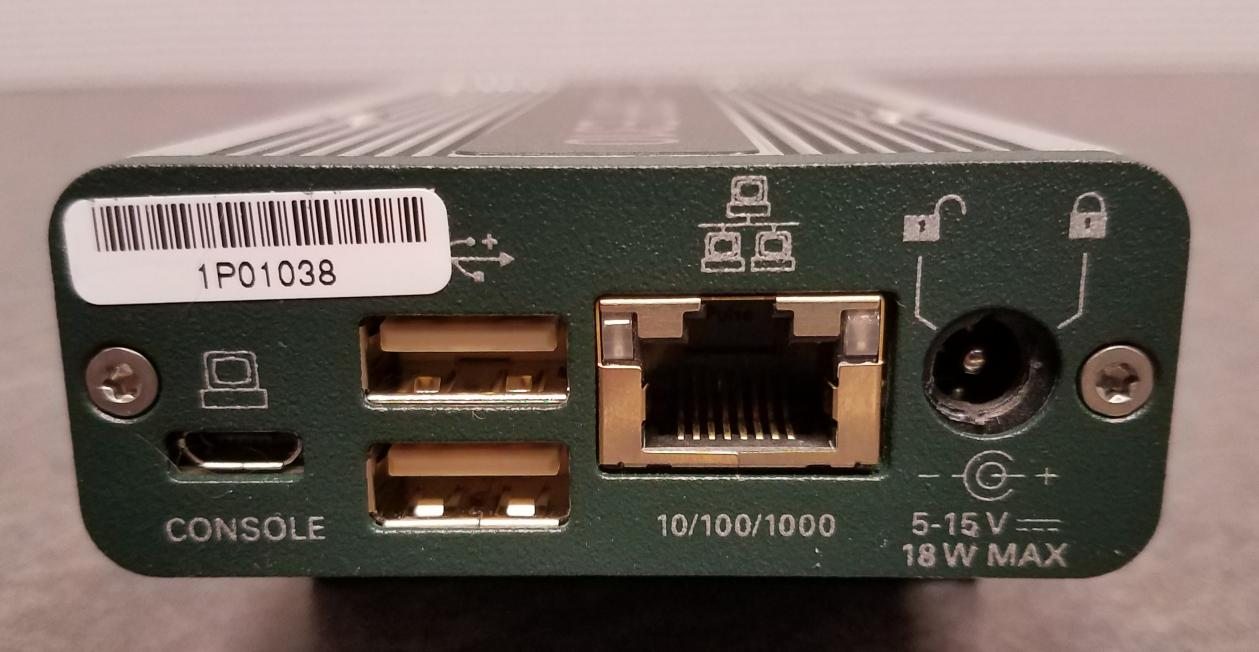
\includegraphics[scale=0.5]{img/back_panel.jpg}
 \caption{Back Panel}
 \label{fig:back}
\end{figure}

\item \textbf{Ethernet cable}:
An Ethernet port is available on the E310 (Figure~\ref{fig:back}) and is required when the Network mode (discussed later) environment is used. The OpenCPI BSP for the E310 is configured for DHCP.\medskip

\begin{figure}[H]
 \centering
 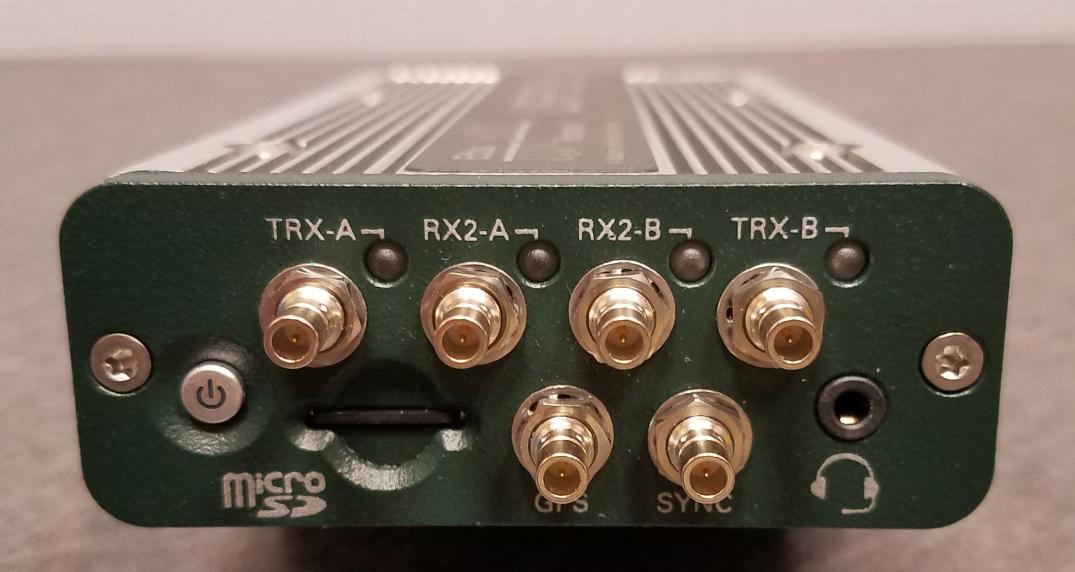
\includegraphics[scale=0.5]{img/front_panel.jpg}
 \caption{Front Panel}
 \label{fig:front}
\end{figure}

\item \textbf{Access to a network which supports DHCP. (Network Mode)}

\item \textbf{SD card}:
As mentioned earlier, a 4GB or larger SD card should come with the SDR. The bootable SD card slot is located on the front of the unit (Figure~\ref{fig:front}) and ejects by gently pushing it in and releasing.

\item \textbf{SD card reader}

\item \textbf{Further information on front panel}:
Also found on the front panel of the SDR are six labeled SMB (50 Ohm) connectors: TRX-A, RX2-A, RX2-B, TRX-B, GPS, and SYNC (Figure~\ref{fig:front}). The upper connections are split into two individual channels referred to as ``Front End A'' and ``Front End B.'' Specific details can be found in the vendor manuals. \\   \bigskip

\end{itemize}
\end{flushleft}

\section{SD Card Setup}
\label{sec:SD_Card_Setup}
\subsection{Make a backup image of factory SD card (assumes Linux host)}
This section provides the steps for creating an SD card backup image. The subsequent subsections assume the SD card is empty.

\begin{itemize}
\item Determine the device file name for the SD card by executing dmesg command below. It will likely be something like \texttt{/dev/sdb} or \texttt{/dev/mmcblk0}.\\
\texttt{\$ dmesg | tail -n 15} \\
\item Run the following dd command to make a backup image, where DEVICENAME was determined above. This step should take $\sim15$ minutes depending on the card size.\\ \medskip
\texttt{\$ dd if=DEVICENAME of=backup.image}
\end{itemize}
\noindent To restore the card back to the original contents, run the command ``\texttt{dd of=DEVICENAME if=backup.image}'' (Do not do this step unless you want the original contents back on the SD card.)

\subsection{Format the SD card}
\begin{itemize}
\item Format the SD card with a single FAT32 partition.
\end{itemize}

\subsection{Copy OpenCPI files to SD card}
This section provides the simplest instructions for copying files over to the SD card. Appendix~\ref{app:sd_card_copy_files} contains more involved instructions for copying \textit{only} the necessary files to the SD card for each mode.\\

\noindent WARNING: The user must ensure that the contents of the SD, match the version of the OpenCPI release that the artifacts were built against.\\

\noindent When using the factory SD card, all files can be ignored or deleted. Any files/directories copied to SD card will appear at \texttt{/mnt/card} on the E310.\\

\noindent Copy the following directory onto the SD card:
\begin{verbatim}
$ cp -rL /opt/opencpi/cdk/e3xx/sdcard-xilinx13_4/* /run/media/<user>/<partition>/
\end{verbatim}

\subsubsection{Copy Standalone Mode specific files to SD card}
Copy the \code{testbias} bitstream into the artifacts directory:
\begin{verbatim}
$ cp /home/ocpi_projects/assets/hdl/assemblies/testbias/container-testbias_e3xx/\
target-zynq/testbias_e3xx_base.bit.gz /run/media/<user>/<partition>/opencpi/xilinx13_4/artifacts
\end{verbatim}

\subsubsection{Copy Network Mode specific files to SD card}
No additional files required for Network Mode.

\subsubsection{SD Card Source}
The final SD Card artifacts are distributed in \path{/opt/opencpi/cdk/e3xx/} via RPM as noted previously. The end user is not required nor expected to generate the files, but the process is documented below in Appendix~\ref{app:sd_card}.

\iffalse
This file is protected by Copyright. Please refer to the COPYRIGHT file
distributed with this source distribution.

This file is part of OpenCPI <http://www.opencpi.org>

OpenCPI is free software: you can redistribute it and/or modify it under the
terms of the GNU Lesser General Public License as published by the Free Software
Foundation, either version 3 of the License, or (at your option) any later
version.

OpenCPI is distributed in the hope that it will be useful, but WITHOUT ANY
WARRANTY; without even the implied warranty of MERCHANTABILITY or FITNESS FOR A
PARTICULAR PURPOSE. See the GNU Lesser General Public License for more details.

You should have received a copy of the GNU Lesser General Public License along
with this program. If not, see <http://www.gnu.org/licenses/>.
\fi


\section{Script Setup}
There are two type of setups or modes for running applications on any embedded radio: Network and Standalone. In Network mode, a development system hosts the OpenCPI tree as an NFS server to the \radioName \space which is an NFS client. This configuration provides quick and dynamic access to all of OpenCPI, and presumably any applications, components and bitstreams. In Standalone mode, all the artifacts are located on the SDR's local storage (\textit{e.g.} SD card) and no network connection is required. This may be more suited for \textit{deployment} scenarios in which network connection is not possible or practical. Network mode is generally preferred during the development process.

\begin{flushleft}

\subsection{Setting up the Network and Standalone Mode scripts}

For each mode, a startup script is used to configure the environment of the embedded system. The OpenCPI framework provides a default script for each mode. The default scripts are to be copied and modified per the user's requirements.\par\medskip

\subsubsection{Network Mode}
1) Make a copy of the default script for editing. \\ \medskip
\begin{texttt}
\$ cp /run/media/<user>/\copyLoc/opencpi/default\_mynetsetup.sh \textbackslash\\
/run/media/<user>/\copyLoc/opencpi/mynetsetup.sh
\end{texttt}\medskip

2) Edit the copy
\begin{enumerate}
\item In \texttt{mynetsetup.sh}, uncomment the following lines which are necessary for mounting \textit{core} and \textit{assets} project: \\ \medskip

\begin{texttt}
mkdir -p \mountPoint ocpi\_core \\
mount -t nfs -o udp,nolock,soft,intr \$1:/home/user/ocpi\_projects/core \mountPoint ocpi\_core \\
mkdir -p \mountPoint ocpi\_assets \\
mount -t nfs -o udp,nolock,soft,intr \$1:/home/user/ocpi\_projects/assets \mountPoint ocpi\_assets\\
\end{texttt}
 \item Edit \texttt{/home/user/ocpi\_projects/core} and \texttt{/home/user/ocpi\_projects/assets} to reflect the paths to the \textit{core} and \textit{assets} project on the host, e.g.:\\ \medskip
\begin{texttt}
mkdir -p \mountPoint ocpi\_core \\
mount -t nfs -o udp,nolock,soft,intr \$1:/home/johndoe/ocpi\_projects/core \mountPoint ocpi\_core\\
mkdir -p \mountPoint ocpi\_assets \\
mount -t nfs -o udp,nolock,soft,intr \$1:/home/johndoe/ocpi\_projects/assets \mountPoint ocpi\_assets\\
\end{texttt}
\ifx\bspProj\undefined
%do nothing 
\else 
\begin{texttt}
mkdir -p \mountPoint \bspProj \\
mount -t nfs -o udp,nolock,soft,intr \$1:/home/johndoe/ocpi\_projects/\bspProj \space \textbackslash \\
\mountPoint \bspProj \\
\end{texttt}
\fi
\end{enumerate}

\subsubsection{Standalone Mode}
In this mode, all OpenCPI artifacts that are required to run any application on the \radioName \space must be copied onto the SD card.  Building the provided projects to obtain such artifacts is discussed in Section \ref{sec:Building OpenCPI projects}. Once the artifacts have been created, they must be copied to the SD card in Section \ref{sec:SD_Card_Setup}. In general, any required \texttt{.so} (RCC workers), \texttt{.bit.gz} (hdl assemblies), and application XMLs or executables must be copied to the ATLAS partition of the SD card. \medskip

1) Make a copy of the default script for editing \\ \medskip
\begin{texttt}
\$ cp /run/media/<user>/\copyLoc/opencpi/default\_mysetup.sh \textbackslash \\
/run/media/<user>/\copyLoc/opencpi/mysetup.sh
\end{texttt}\medskip

2) Edit the copy \\ \medskip
Unlike Network mode, there is no required modifications to this script. \medskip

3) Copy any additional artifacts to SD card's \texttt{opencpi/\rccplatform/artifacts/} directory \medskip




\iffalse
This file is protected by Copyright. Please refer to the COPYRIGHT file
distributed with this source distribution.

This file is part of OpenCPI <http://www.opencpi.org>

OpenCPI is free software: you can redistribute it and/or modify it under the
terms of the GNU Lesser General Public License as published by the Free Software
Foundation, either version 3 of the License, or (at your option) any later
version.

OpenCPI is distributed in the hope that it will be useful, but WITHOUT ANY
WARRANTY; without even the implied warranty of MERCHANTABILITY or FITNESS FOR A
PARTICULAR PURPOSE. See the GNU Lesser General Public License for more details.

You should have received a copy of the GNU Lesser General Public License along
with this program. If not, see <http://www.gnu.org/licenses/>.
\fi

% This is for inserting into various "Getting Started" Guides
% First, turn off indenting to avoid all the flushleft
\newlength{\savedparindentsystime}%
\setlength{\savedparindentsystime}{\parindent}%
\setlength{\parindent}{0pt} % Don't indent all paragraphs
\providecommand{\forceindent}{\leavevmode{\parindent=1em\indent}}%
\subsection{Setup system time reference}
\label{sec:Setup system time reference}
\textbf{If Linux system time is not required to be accurate, this step may be skipped.} \\ \medskip

\textit{For either Network or Standalone mode}, the following settings that are passed by \texttt{mynetsetup.sh/mysetup.sh} to the \texttt{zynq\_net\_setup.sh/zynq\_setup.sh} scripts \textit{may} require modification:

\begin{itemize}
 \item Identify the system that is to be used as a time server, where the default is ``time.nist.gov'' and is set in \path{/mnt/card/opencpi/ntp.conf}. A valid time server must support ntp.
 \item Identify the current timezone description, where the default is ``EST5EDT,M3.2.0,M11.1.0''. Change this if required for the local timezone. See \texttt{man tzset} on the host PC for more information.
 \item If a time server is not required, or cannot connect to a time server, the user is required to manually set the time at start up.  Use the \code{date} command to manually set the Linux system time. See \texttt{man date} on the host PC for more information.
\end{itemize}
\setlength{\parindent}{\savedparindentsystime}%

\iffalse
This file is protected by Copyright. Please refer to the COPYRIGHT file
distributed with this source distribution.

This file is part of OpenCPI <http://www.opencpi.org>

OpenCPI is free software: you can redistribute it and/or modify it under the
terms of the GNU Lesser General Public License as published by the Free Software
Foundation, either version 3 of the License, or (at your option) any later
version.

OpenCPI is distributed in the hope that it will be useful, but WITHOUT ANY
WARRANTY; without even the implied warranty of MERCHANTABILITY or FITNESS FOR A
PARTICULAR PURPOSE. See the GNU Lesser General Public License for more details.

You should have received a copy of the GNU Lesser General Public License along
with this program. If not, see <http://www.gnu.org/licenses/>.
\fi

% This is for inserting into various "Getting Started" Guides
% First, turn off indenting to avoid all the flushleft
\newlength{\savedparindentrsync}%
\setlength{\savedparindentrsync}{\parindent}%
\setlength{\parindent}{0pt} % Don't indent all paragraphs
\providecommand{\forceindent}{\leavevmode{\parindent=1em\indent}}%
\def\qrsync{``\code{rsync}''~}
\subsection{\qrsync provided binary}
\label{sec:rsync}
An ARM-compiled version of \qrsync is provided in the included SD card image for \rccplatform.
This tool allows the use of \textit{standalone mode} while shortening the required developer time to synchronize the artifacts being developed.
For command-line usage, see the \href{https://rsync.samba.org/documentation.html}{rsync home page}.
The easiest usage is to have the radio ``pull'' from the developer's workstation; this does not need any additional command-line arguments.
\subsubsection*{Implementation Details}
Unfortunately, the \qrsync executable is not in the default path because when called remotely, it requests a non-interactive shell. For this reason, a ``pull'' approach is recommended.
If a user for some reason requires a ``push'' from the workstation to the radio, the local \qrsync executable must be told the \textit{remote location} of the \path{rsync} executable to call, \textit{e.g.} \code{rsync --rsync-path=/mnt/card/opencpi/\rccplatform/bin/rsync}
\setlength{\parindent}{\savedparindentrsync}%

\end{flushleft}

\section{Development Host Setup - Network Mode ONLY}

% Bring in NFS setup snippet (has subsections)
\iffalse
This file is protected by Copyright. Please refer to the COPYRIGHT file
distributed with this source distribution.

This file is part of OpenCPI <http://www.opencpi.org>

OpenCPI is free software: you can redistribute it and/or modify it under the
terms of the GNU Lesser General Public License as published by the Free Software
Foundation, either version 3 of the License, or (at your option) any later
version.

OpenCPI is distributed in the hope that it will be useful, but WITHOUT ANY
WARRANTY; without even the implied warranty of MERCHANTABILITY or FITNESS FOR A
PARTICULAR PURPOSE. See the GNU Lesser General Public License for more details.

You should have received a copy of the GNU Lesser General Public License along
with this program. If not, see <http://www.gnu.org/licenses/>.
\fi
% Any changes to this document should be made in opencpi.git

% This is for inserting into various "Getting Started" Guides
% First, turn off indenting to avoid all the flushleft
\newlength{\savedparindentnfs}%
\setlength{\savedparindentnfs}{\parindent}%
\setlength{\parindent}{0pt} % Don't indent all paragraphs
\providecommand{\forceindent}{\leavevmode{\parindent=1em\indent}}%

\subsection{Network Mounting Mode}
\label{sec:network_mode}
The NFS server needs to be enabled on the host in order to run the SDR in Network Mode. The following sections are directions on how to do this for both CentOS~6 and CentOS~7 host operating systems.
\subsubsection{CentOS~6}
% \begin{minipage}{\linewidth}
From the host, install the necessary tools using yum:
\begin{verbatim}
% sudo yum install nfs-utils nfs-utils-lib
% sudo chkconfig nfs on
% sudo service rpcbind start
% sudo service nfs start
\end{verbatim}
% \end{minipage}
% ~\\

% \begin{minipage}{\linewidth}
From the host, add the following lines to the bottom of \texttt{/etc/exports} and change ``XX.XX.XX.XX/MM'' to a valid netmask for the DHCP range that the SDR will be set to for your network (\textit{e.g.} \texttt{192.168.0.0/16}).
\begin{verbatim}
% sudo vi /etc/exports

/opt/opencpi XX.XX.XX.XX/MM(rw,sync,no_root_squash,no_subtree_check)
<host core project location> XX.XX.XX.XX/MM(rw,sync,no_root_squash,no_subtree_check)
<host assets project location> XX.XX.XX.XX/MM(rw,sync,no_root_squash,no_subtree_check)

% sudo exportfs -av
\end{verbatim}
% \end{minipage}
% ~\\

% \begin{minipage}{\linewidth}
From the host, restart the services that have modified for the changes to take effect:
\begin{verbatim}
% sudo service nfs start
\end{verbatim}
% \end{minipage}

\subsubsection{CentOS~7}
% \begin{minipage}{\linewidth}
From the host, install the necessary tools using yum:\\
~\\
\verb+% sudo yum install nfs-utils+ \footnote{\texttt{nfs-utils-lib} was rolled into \texttt{nfs-utils} starting with CentOS 7.2, if using eariler versions of CentOS 7, \texttt{nfs-utils-lib} will need to be explicitly installed}
% \end{minipage}
~\\

% \begin{minipage}{\linewidth}
From the host, allow NFS past SELinux\footnote{You can use \texttt{getsebool} to see if these values are already set before attempting to set them. Some security tools may interpret the change attempt as a system attack.}:
\begin{verbatim}
% sudo setsebool -P nfs_export_all_rw 1
% sudo setsebool -P use_nfs_home_dirs 1
\end{verbatim}
% \end{minipage}
% ~\\

% \begin{minipage}{\linewidth}
From the host, allow NFS past the firewall:
\begin{verbatim}
% sudo firewall-cmd --permanent --zone=public --add-service=nfs
% sudo firewall-cmd --permanent --zone=public --add-port=2049/udp
% sudo firewall-cmd --permanent --zone=public --add-service=mountd
% sudo firewall-cmd --permanent --zone=public --add-service=rpc-bind
% sudo firewall-cmd --reload
\end{verbatim}
% \end{minipage}
% ~\\

% \begin{minipage}{\linewidth}
Define the export by creating a new file that has the extension ``\texttt{exports}''. If it does not have that extension, it will be ignored.  Add the following lines to that file and replace ``XX.XX.XX.XX/MM'' with a valid netmask for the DHCP range that the SDR will be set to for your network (\textit{e.g.} \texttt{192.168.0.0/16}).
\begin{verbatim}
% sudo vi /etc/exports.d/user_ocpi.exports

/opt/opencpi XX.XX.XX.XX/MM(rw,sync,no_root_squash,crossmnt)
/home/user/ocpi_projects/core XX.XX.XX.XX/MM(rw,sync,no_root_squash,crossmnt)
/home/user/ocpi_projects/assets XX.XX.XX.XX/MM(rw,sync,no_root_squash,crossmnt)
\end{verbatim}
% \end{minipage}
% ~\\

% \begin{minipage}{\linewidth}
If the file system that you are mounting is XFS, then each mount needs to have a unique \texttt{fsid} defined. Instead, use:
\begin{verbatim}
% sudo vi /etc/exports.d/user_ocpi.exports

/opt/opencpi XX.XX.XX.XX/MM(rw,sync,no_root_squash,crossmnt,fsid=33)
/home/user/ocpi_projects/core XX.XX.XX.XX/MM(rw,sync,no_root_squash,crossmnt,fsid=34)
/home/user/ocpi_projects/assets XX.XX.XX.XX/MM(rw,sync,no_root_squash,crossmnt,fsid=35)
\end{verbatim}
% \end{minipage}
% ~\\

% \begin{minipage}{\linewidth}
Restart the services that have modified for the changes to take effect:
\begin{verbatim}
% sudo systemctl enable rpcbind
% sudo systemctl enable nfs-server
% sudo systemctl enable nfs-lock
% sudo systemctl enable nfs-idmap
% sudo systemctl restart rpcbind
% sudo systemctl restart nfs-server
% sudo systemctl restart nfs-lock
% sudo systemctl restart nfs-idmap
\end{verbatim}
% \end{minipage}
% ~\\

* Note: Some of the ``enable'' commands may fail based on your package selection, but should not cause any problems.
\setlength{\parindent}{\savedparindentnfs}%

%
\\\\NOTE: You will need to add the \code{ocpi.bsp.e310} project to your list of exports (in \path{/etc/exports.d/user_ocpi.exports}).

\pagebreak
\section{Configuring the runtime environment on the platform}

\subsection{Network Mode}
\begin{enumerate}
\item Plug in an Ethernet cable to a network configured for DHCP
\item Ensure a micro-USB to USB cable is connected between the E310's serial port and development host
\item Apply power to the E310
\item Use a serial terminal application to establish a serial connection, for example:

\begin{verbatim}
$ sudo screen /dev/ttyUSB0 115200
\end{verbatim}

\item After a successful boot to PetaLinux, login to the system, using  ``\textbf{root}'' for user name and password

\item Setup the OpenCPI environment on remote system

\begin{flushleft}
Each time the SDR is booted, the OpenCPI environment must be setup. By sourcing the \texttt{mynetsetup.sh} script, the remote system's environment is configured for OpenCPI and NFS directories are mounted for Network mode.\footnote{This script calls the \texttt{zynq\_net\_setup.sh} script, which should not be modifiable by the user.}. The user must provide the network address of the development system to the script as its only argument:
\begin{verbatim}
$ . /mnt/card/opencpi/mynetsetup.sh XX.XX.XX.XX
\end{verbatim}

where XX.XX.XX.XX is the IP address of the NFS host (i.e. that development host, \textit{e.g.} 192.168.1.10). A successful run should output the following:
\begin{verbatim}
An IP address was detected.
Setting the time from time server: time.nist.gov
My IP address is: XX.XX.XX.XX, and my hostname is: zynq
Running login script. OCPI_CDK_DIR is now /mnt/net/cdk.
Executing /home/root/.profile
No reserved DMA memory found on the linux boot command line.
The mdev config has no OpenCPI rules. We will add them to /etc/mdev.conf
NET: Registered protocol family 12
Driver loaded successfully.
OpenCPI ready for zynq.
Discovering available containers...
Available containers:
 #  Model Platform       OS     OS-Version  Arch     Name
 0  hdl   e3xx                                       PL:0
 1  rcc   xilinx13_4     linux  x13_4       arm      rcc0
\end{verbatim}
\iffalse
This file is protected by Copyright. Please refer to the COPYRIGHT file
distributed with this source distribution.

This file is part of OpenCPI <http://www.opencpi.org>

OpenCPI is free software: you can redistribute it and/or modify it under the
terms of the GNU Lesser General Public License as published by the Free Software
Foundation, either version 3 of the License, or (at your option) any later
version.

OpenCPI is distributed in the hope that it will be useful, but WITHOUT ANY
WARRANTY; without even the implied warranty of MERCHANTABILITY or FITNESS FOR A
PARTICULAR PURPOSE. See the GNU Lesser General Public License for more details.

You should have received a copy of the GNU Lesser General Public License along
with this program. If not, see <http://www.gnu.org/licenses/>.
\fi

% This is for inserting into various "Getting Started" Guides
% First, turn off indenting to avoid all the flushleft
%\newlength{\savedparindentntp}%
%\setlength{\savedparindentntp}{\parindent}%
%\setlength{\parindent}{0pt} % Don't indent all paragraphs
%\providecommand{\forceindent}{\leavevmode{\parindent=1em\indent}}%
Note: If the output includes:
\begin{verbatim}
Attempting to set the time from time server
Alarm clock
\end{verbatim}
\path{ntp} was unable to set time using servers in \path{ntp.conf}. For more information see Section \ref{sec:Setup system time reference}

%\setlength{\parindent}{\savedparindentntp}%

\end{flushleft}
\end{enumerate}

\pagebreak
\subsection{Standalone Mode}
\begin{enumerate}
\item (Not required for OpenCPI in this mode) Plug in an Ethernet cable to a network configured for DHCP
\item Ensure a micro-USB to USB cable is connected between the E310's serial port and development host
\item Apply power to the E310
\item Use a serial terminal application to establish a serial connection, for example:

\begin{verbatim}
$ sudo screen /dev/ttyUSB0 115200
\end{verbatim}

\item After a successful boot to PetaLinux, login to the system, using  ``\textbf{root}'' for user name and password

\item \textcolor{red}{WARNING:}
Applications (including XML-only ones) fail if there is not an IP address assigned to the platform, even when in ``standalone mode.'' When the Ethernet port is not connected to a network configured with DHCP, a temporary IP address must be set:
\begin{verbatim}
$ ifconfig eth0 192.168.244.244
\end{verbatim} \medskip

\item Setup the OpenCPI environment on remote system

\begin{flushleft}
Each time the SDR is booted, the OpenCPI environment must be setup. By sourcing the \texttt{mysetup.sh} script, the remote system's environment is configured for OpenCPI \footnote{This script calls the \texttt{zynq\_setup.sh} script, which should not be modifiable by the user.}. There are no arguments for this script.
\begin{verbatim}
$ . /mnt/card/opencpi/mysetup.sh
\end{verbatim}

A successful run should output the following:
\begin{verbatim}
Attempting to set the time from time server: time.nist.gov
Setting the time from time server: time.nist.gov
Running login script. OCPI_CDK_DIR is now /mnt/card/opencpi.
Executing /home/root/.profile
No reserved DMA memory found on the linux boot command line.
The mdev config has no OpenCPI rules. We will add them to /etc/mdev.conf
NET: Registered protocol family 12
Driver loaded successfully.
OpenCPI ready for zynq.
Discovering available containers...
Available containers:
 #  Model Platform       OS     OS-Version  Arch     Name
 0  hdl   e3xx                                       PL:0
 1  rcc   xilinx13_4     linux  x13_4       arm      rcc0
\end{verbatim}
\iffalse
This file is protected by Copyright. Please refer to the COPYRIGHT file
distributed with this source distribution.

This file is part of OpenCPI <http://www.opencpi.org>

OpenCPI is free software: you can redistribute it and/or modify it under the
terms of the GNU Lesser General Public License as published by the Free Software
Foundation, either version 3 of the License, or (at your option) any later
version.

OpenCPI is distributed in the hope that it will be useful, but WITHOUT ANY
WARRANTY; without even the implied warranty of MERCHANTABILITY or FITNESS FOR A
PARTICULAR PURPOSE. See the GNU Lesser General Public License for more details.

You should have received a copy of the GNU Lesser General Public License along
with this program. If not, see <http://www.gnu.org/licenses/>.
\fi

% This is for inserting into various "Getting Started" Guides
% First, turn off indenting to avoid all the flushleft
%\newlength{\savedparindentntp}%
%\setlength{\savedparindentntp}{\parindent}%
%\setlength{\parindent}{0pt} % Don't indent all paragraphs
%\providecommand{\forceindent}{\leavevmode{\parindent=1em\indent}}%
Note: If the output includes:
\begin{verbatim}
Attempting to set the time from time server
Alarm clock
\end{verbatim}
\path{ntp} was unable to set time using servers in \path{ntp.conf}. For more information see Section \ref{sec:Setup system time reference}

%\setlength{\parindent}{\savedparindentntp}%

\end{flushleft}
\end{enumerate}

\pagebreak
\section{Build an application}
\begin{flushleft}
The setup of the platform can be verified by running an application that uses both RCC and HDL workers. A simple application that requires two RCC and one HDL worker is located in \texttt{assets/applications/bias.xml}, but only the RCC artifacts are provided with the installation of RPMs, and are availble on the SD card (Standard Mode) or mounted CDK directory (Network Mode). The remaining task is to build an assembly, or bitstream for loading the FPGA, which contains the HDL worker.
\end{flushleft}

\section{Run an Application}
\subsection{Network Mode}
 \label{sec:ocpirun_net}
The default setup script sets the \texttt{OCPI\_LIBRARY\_PATH} variable to include the RCC workers that are required to execute the application, but it must be updated to include to the assembly bitstream that was built.  After running the \texttt{mynetsetup.sh} script, navigate to  \texttt{/mnt/ocpi\_assets/applications}, then update the \texttt{OCPI\_LIBRARY\_PATH} variable using the following command:
\begin{verbatim}
$ export OCPI_LIBRARY_PATH=/mnt/ocpi_assets/artifacts:/mnt/ocpi_core/artifacts
\end{verbatim}
Run the application using the following command:
\begin{verbatim}
$ ocpirun -v -t 1 -d -m bias=hdl bias.xml
\end{verbatim}
The output should be similar to:
\begin{lstlisting}[showspaces=false]
Available containers are:  0: PL:0 [model: hdl os:  platform: e3xx], 1: rcc0 [model: rcc os: linux platform: xilinx13_4]
Actual deployment is:
  Instance  0 file_read (spec ocpi.core.file_read) on rcc container 1: rcc0, using file_read in /mnt/ocpi_core/artifacts/ocpi.core.file_read.rcc.0.xilinx13_4.so dated Fri Sep 28 18:18:26 2018
  Instance  1 bias (spec ocpi.core.bias) on hdl container 0: PL:0, using bias_vhdl/a/bias_vhdl in /mnt/ocpi_assets/artifacts/ocpi.assets.testbias_e3xx_base.hdl.0.e3xx.gz dated Tue Oct  2 11:59:53 2018
  Instance  2 file_write (spec ocpi.core.file_write) on rcc container 1: rcc0, using file_write in /mnt/ocpi_core/artifacts/ocpi.core.file_write.rcc.0.xilinx13_4.so dated Fri Sep 28 18:18:31 2018
Application XML parsed and deployments (containers and artifacts) chosen
Application established: containers, workers, connections all created
Communication with the application established
Dump of all initial property values:
Property  0: file_read.fileName = "test.input" (cached)
Property  1: file_read.messagesInFile = "false" (cached)
Property  2: file_read.opcode = "0" (cached)
Property  3: file_read.messageSize = "16"
Property  4: file_read.granularity = "4" (cached)
Property  5: file_read.repeat = "<unreadable>"
Property  6: file_read.bytesRead = "0"
Property  7: file_read.messagesWritten = "0"
Property  8: file_read.suppressEOF = "false"
Property  9: file_read.badMessage = "false"
Property 10: file_read.ocpi_debug = "false" (parameter)
Property 11: file_read.ocpi_endian = "little" (parameter)
Property 12: bias.biasValue = "16909060" (cached)
Property 13: bias.ocpi_debug = "false" (parameter)
Property 14: bias.ocpi_endian = "little" (parameter)
Property 15: bias.test64 = "0"
Property 16: file_write.fileName = "test.output" (cached)
Property 17: file_write.messagesInFile = "false" (cached)
Property 18: file_write.bytesWritten = "0"
Property 19: file_write.messagesWritten = "0"
Property 20: file_write.stopOnEOF = "true" (cached)
Property 21: file_write.ocpi_debug = "false" (parameter)
Property 22: file_write.ocpi_endian = "little" (parameter)
Application started/running
Waiting up to 1 seconds for application to finish
Application finished
Dump of all final property values:
Property  3: file_read.messageSize = "16"
Property  5: file_read.repeat = "<unreadable>"
Property  6: file_read.bytesRead = "4000"
Property  7: file_read.messagesWritten = "251"
Property  8: file_read.suppressEOF = "false"
Property  9: file_read.badMessage = "false"
Property 15: bias.test64 = "0"
Property 18: file_write.bytesWritten = "4000"
Property 19: file_write.messagesWritten = "250"
\end{lstlisting}

\noindent Run the following command to view the input:
\begin{verbatim}
$ hexdump test.input | less
\end{verbatim}
 The output should look like the following:
\begin{verbatim}
0000000 0000 0000 0001 0000 0002 0000 0003 0000
0000010 0004 0000 0005 0000 0006 0000 0007 0000
0000020 0008 0000 0009 0000 000a 0000 000b 0000
0000030 000c 0000 000d 0000 000e 0000 000f 0000
0000040 0010 0000 0011 0000 0012 0000 0013 0000
0000050 0014 0000 0015 0000 0016 0000 0017 0000
0000060 0018 0000 0019 0000 001a 0000 001b 0000
0000070 001c 0000 001d 0000 001e 0000 001f 0000
0000080 0020 0000 0021 0000 0022 0000 0023 0000
0000090 0024 0000 0025 0000 0026 0000 0027 0000
00000a0 0028 0000 0029 0000 002a 0000 002b 0000
00000b0 002c 0000 002d 0000 002e 0000 002f 0000
00000c0 0030 0000 0031 0000 0032 0000 0033 0000
00000d0 0034 0000 0035 0000 0036 0000 0037 0000
00000e0 0038 0000 0039 0000 003a 0000 003b 0000
00000f0 003c 0000 003d 0000 003e 0000 003f 0000
0000100 0040 0000 0041 0000 0042 0000 0043 0000
0000110 0044 0000 0045 0000 0046 0000 0047 0000
0000120 0048 0000 0049 0000 004a 0000 004b 0000
0000130 004c 0000 004d 0000 004e 0000 004f 0000
0000140 0050 0000 0051 0000 0052 0000 0053 0000
0000150 0054 0000 0055 0000 0056 0000 0057 0000
0000160 0058 0000 0059 0000 005a 0000 005b 0000
\end{verbatim}

\noindent Run the following command to view the output: \\
\begin{verbatim}
$ hexdump test.output | less
\end{verbatim}\medskip
 The output should look like the following:
\begin{verbatim}
0000000 0304 0102 0305 0102 0306 0102 0307 0102
0000010 0308 0102 0309 0102 030a 0102 030b 0102
0000020 030c 0102 030d 0102 030e 0102 030f 0102
0000030 0310 0102 0311 0102 0312 0102 0313 0102
0000040 0314 0102 0315 0102 0316 0102 0317 0102
0000050 0318 0102 0319 0102 031a 0102 031b 0102
0000060 031c 0102 031d 0102 031e 0102 031f 0102
0000070 0320 0102 0321 0102 0322 0102 0323 0102
0000080 0324 0102 0325 0102 0326 0102 0327 0102
0000090 0328 0102 0329 0102 032a 0102 032b 0102
00000a0 032c 0102 032d 0102 032e 0102 032f 0102
00000b0 0330 0102 0331 0102 0332 0102 0333 0102
00000c0 0334 0102 0335 0102 0336 0102 0337 0102
00000d0 0338 0102 0339 0102 033a 0102 033b 0102
00000e0 033c 0102 033d 0102 033e 0102 033f 0102
00000f0 0340 0102 0341 0102 0342 0102 0343 0102
0000100 0344 0102 0345 0102 0346 0102 0347 0102
0000110 0348 0102 0349 0102 034a 0102 034b 0102
0000120 034c 0102 034d 0102 034e 0102 034f 0102
0000130 0350 0102 0351 0102 0352 0102 0353 0102
0000140 0354 0102 0355 0102 0356 0102 0357 0102
0000150 0358 0102 0359 0102 035a 0102 035b 0102
0000160 035c 0102 035d 0102 035e 0102 035f 0102
\end{verbatim}

\newpage
\subsection{Run an Application in Standalone Mode}
\begin{flushleft}
The default setup script sets the \texttt{OCPI\_LIBRARY\_PATH} variable to include the all of the artifacts that are required to execute the application. Specifically, all three of the artifacts that are located on the SD card are mounted at \texttt{/mnt/card/opencpi/xilinx13\_4/artifacts}.  After running \texttt{mysetup.sh}, navigate to \texttt{/mnt/card/opencpi/xml}.

Run the application using the following command:
\begin{verbatim}
$ ocpirun -v -t 1 -d -m bias=hdl bias.xml
\end{verbatim}
The output should be similar to the output shown in Section~\ref{sec:ocpirun_net}.
\end{flushleft}

\noindent Run the following commands to view the input and output, and reference Section~\ref{sec:ocpirun_net} for the expected results: \\
\begin{verbatim}
$ hexdump test.input | less
\end{verbatim}
\begin{verbatim}
$ hexdump test.output | less
\end{verbatim}

\section{Running Reference Applications}
Now that you have set up OpenCPI and the E310 radio, you can run one of the reference applications. Navigate to \code{bsp\_e310/applications/FSK} or \code{bsp\_e310/applications/rx\_app} and follow the instructions in the corresponding documents (\textit{FSK\_App\_Getting\_Started\_Guide\_E3XX.pdf} and \textit{FSK\_app\_e3xx.pdf}, or \textit{RX\_app\_e3xx.pdf}).
\newpage

\begin{appendices}
\section{Generating Boot Artifacts}
\label{app:sd_card}
In normal use cases, the SD card should be createdable and usable via the simple steps in Section~\ref{sec:SD_Card_Setup}. This section outlines the steps required to regenerate the artifacts used in previous sections for solely informational purposes and is not expected for users to have to complete these steps.
\subsection{BOOT.bin and u-boot.img}
The original first and second stage bootloader artifacts that come installed on the E310 SD card are not suitable for the Petalinux build OpenCPI uses for its software platform as those artifacts are expecting a uImage kernel with a separate filesystem partition, while the Petalinux build uses a separate ramdisk image file. The \path{BOOT.bin} and \path{u-boot.img} files were rebuilt in order to support booting into this style of Linux images from Ettus's and Xilinx's repositories. In summary, the repositories were cloned and checked out to the proper branch, according to the release for the e310 and the bitbake recipe, and subsequently cross-compiled for ARM using the Xilinx toolchain. The steps are shown below.
\begin{lstlisting}[showspaces=false]
$ git clone https://github.com/EttusResearch/meta-ettus.git
$ cd meta-ettus && git checkout e300-daisy && cd ..
$ git clone https://github.com/Xilinx/u-boot-xlnx.git
$ cd u-boot-xlnx && git checkout 664820b231b129552e963e1a96b45ac7196ccc81 && cd ..
$ cp meta-ettus/e300-bsp/recipes-bsp/u-boot/ettus-e300/* u-boot-xlnx/
$ cd u-boot-xlnx
$ mv ps7_init.{c,h} board/xilinx/zynq/
$ git apply 0001-E300-Uses-UART0-for-console.patch
$ git apply 0002-E300-Disable-QSPI.patch
$ git apply 0003-Read-mac-address-from-i2c-EEPROM.patch
$ git apply 0001-e300-Added-memory-test.patch
$ source {xilinx-install-dir}/Xilinx/SDK/2013.4/settings64.sh
$ make zynq_zc70x_config CROSS_COMPILE=arm-xilinx-linux-gnueabi-
$ make CROSS_COMPILE=arm-xilinx-linux-gnueabi-
\end{lstlisting}
\subsection{devicetree.dtb}
The device tree needed to be modified in order to register the hardware devices with the correct hardware device driver in the Petalinux kernel. In summary, the device tree provided by Ettus was decompiled to a device tree source (\path{dts}) file using the device tree compiler (\path{dtc}), modified the text file by adding the proper "compatible" strings to the devices, and subsequently compiled back into a device tree blob (\path{dtb}). The steps shown below assume \path{dtc} is in your \path{$PATH} and the original device tree blob is in the current working directory.
\begin{lstlisting}[showspaces=false]
$ dtc -I dtb -O dts -o devicetree.dts uImage-zynq-e31x-3.dtb
$ vim devicetree.dts
$ dtc -I dts -O dtb -o devicetree.dtb devicetree.dts
\end{lstlisting}
Note: The full source for the modified devicetree.dts can be found at
\path{<BSP project>/hdl/platforms/e3xx/sd_card_source/devicetree.dts}

\subsection{uImage and uramdisk.image.gz}
The \path{uImage} and \path{uramdisk.image.gz} image files come directly from the default 13\_4 OpenCPI software platform. The 13\_3 software platform could not be used due to the SD card driver in 13\_3 not supporting the E310's SD card device.

\section{Copying only required files to SD card}
\label{app:sd_card_copy_files}

\subsection{Copy embedded OS and boot files to SD card}
\label{sec:Copy embedded OS and boot files to SD card}
\noindent Copy the following files/directories onto the SD card:
\begin{verbatim}
$ cp /opt/opencpi/cdk/e3xx/sdcard-xilinx13_4/boot.bin /run/media/<user>/<partition>/

$ cp /opt/opencpi/cdk/e3xx/sdcard-xilinx13_4/devicetree.dtb /run/media/<user>/<partition>/

$ cp /opt/opencpi/cdk/e3xx/sdcard-xilinx13_4/u-boot.img /run/media/<user>/<partition>/

$ cp /opt/opencpi/cdk/e3xx/sdcard-xilinx13_4/uImage /run/media/<user>/<partition>/

$ cp /opt/opencpi/cdk/e3xx/sdcard-xilinx13_4/uramdisk.image.gz /run/media/<user>/<partition>/
\end{verbatim}\medskip

\subsection{Files needed for Standalone Mode}
After performing the steps from \ref{sec:Copy embedded OS and boot files to SD card}, copy the entire \textit{opencpi} directory to the SD card, then copy the relevant bitstreams, artifacts into the \textit{artifacts} directory and application XMLs into the \textit{applications} directory. For this getting started guide, only one bitstream is required to be copied onto the SD cards, where as the required artifacts and application XML where copied to the SD along with the entire \textit{opencpi} directory.

\begin{verbatim}

$ cp -rL /opt/opencpi/cdk/e3xx/sdcard-xilinx13_4/opencpi /run/media/<user>/<partition>/

$ cp /home/<user>/ocpi_projects/assets/hdl/assemblies/testbias/container-testbias_e3xx_base/\
target-zynq/testbias_e3xx_base.bit.gz /run/media/<user>/<partition>/opencpi/xilinx13_4/artifacts
\end{verbatim}

\subsection{Files needed for Network Mode}
After performing the steps from \ref{sec:Copy embedded OS and boot files to SD card}, create a directory on the partition named "opencpi" and copy the following files into the this directory:

\begin{verbatim}
$ mkdir /run/media/<user>/<partition>/opencpi

$ cp /opt/opencpi/cdk/e3xx/sdcard-xilinx13_4/opencpi/default_mynetsetup.sh \
/run/media/<user>/<partition>/opencpi/

$ cp /opt/opencpi/cdk/e3xx/sdcard-xilinx13_4/opencpi/zynq_net_setup.sh \
/run/media/<user>/<partition>/opencpi/
\end{verbatim}

\end{appendices}



\end{document}
